% slides.tex — Beamer presentation for Q4 project
% Audience: postgraduate students in Algorithms in Structural Bioinformatics
% Compile: pdflatex slides.tex  (twice)
\documentclass[aspectratio=169, 10pt]{beamer}

\usetheme{Madrid}
\usecolortheme{whale}
\setbeamertemplate{navigation symbols}{}
\setbeamertemplate{footline}[frame number]

\usepackage{amsmath,amssymb}
\usepackage{graphicx}
\usepackage{booktabs}
\usepackage{tikz}
\usetikzlibrary{shapes.geometric, arrows.meta, positioning, calc, decorations.pathreplacing, fit, backgrounds}
\usepackage{xcolor}
\usepackage{multicol}

% ── Colour palette ────────────────────────────────────────────────────────────
\definecolor{highhp}{RGB}{31,119,180}   % ordered / high confidence
\definecolor{lowhp}{RGB}{214,39,40}     % disordered / low confidence
\definecolor{mixhp}{RGB}{44,160,44}     % mixed / moderate
\definecolor{accentgold}{RGB}{255,185,0}
\definecolor{pipeboxbg}{RGB}{235,245,255}
\definecolor{pipeboxborder}{RGB}{70,130,180}

% ── Title info ────────────────────────────────────────────────────────────────
\title[pLDDT Fragmentation via TDA]{%
  Topological Analysis of pLDDT Profiles:\\[4pt]
  Reproducing and Extending Cazals \& Sarti (2025)%
}
\subtitle{Algorithms in Structural Bioinformatics — Q4 Project}
\author{Giorgos Boulogeorgos}
\institute{Supervisor: Professor I. Emiris \and Co-advisor: P. Rigas}
\date{May 2026}

% ─────────────────────────────────────────────────────────────────────────────
\begin{document}

% ── Title slide ───────────────────────────────────────────────────────────────
\begin{frame}
  \titlepage
\end{frame}

% ── Outline ───────────────────────────────────────────────────────────────────
\begin{frame}{Outline}
  \tableofcontents[hideallsubsections]
\end{frame}

% =============================================================================
\section{Motivation}
% =============================================================================

\begin{frame}{What is pLDDT and why does its \emph{structure} matter?}
  \begin{columns}[T]
    \begin{column}{0.52\textwidth}
      \textbf{pLDDT} (predicted Local Distance Difference Test)
      \begin{itemize}\setlength{\itemsep}{0pt}
        \item Per-residue confidence score, $s_i \in [0, 100]$
        \item Stored in the B-factor column of AlphaFold PDB files
        \item $s_i \gtrsim 70$: well-folded region
        \item $s_i \lesssim 50$: intrinsically disordered
      \end{itemize}
      \vspace{2pt}
      \textbf{Key observation}
      \begin{itemize}\setlength{\itemsep}{0pt}
        \item Most analyses use pLDDT as a \emph{threshold} (keep/discard)
        \item \textbf{Cazals \& Sarti (2025)} treat the full pLDDT
              \emph{profile along the chain} as a topological object
        \item This encodes multi-domain and disordered-linker structure
      \end{itemize}
    \end{column}
    \begin{column}{0.45\textwidth}
      % Schematic pLDDT profile — pure TikZ, x:0-50 y:0-105
      \vspace{-4pt}
      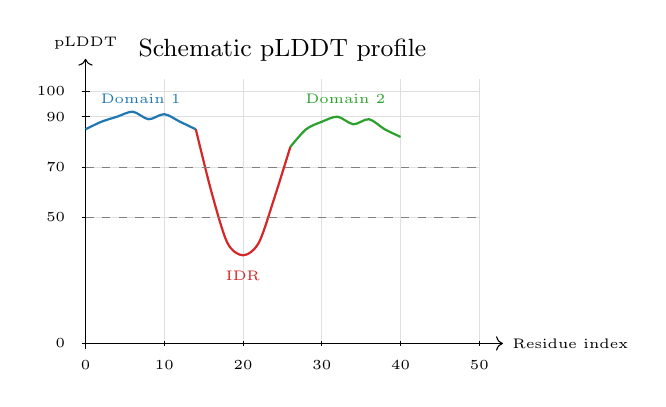
\begin{tikzpicture}[x=0.10cm, y=0.032cm]
        % Light grid
        \foreach \y in {50,70,90,100}
          \draw[gray!25,thin] (0,\y) -- (50,\y);
        \foreach \x in {10,20,30,40,50}
          \draw[gray!25,thin] (\x,0) -- (\x,105);
        % Axes
        \draw[->] (-0.5,0) -- (53,0) node[right,font=\tiny] {Residue index};
        \draw[->] (0,-2) -- (0,113) node[above,font=\tiny] {pLDDT};
        % X ticks
        \foreach \x in {0,10,20,30,40,50} {
          \draw (\x,-1) -- (\x,1);
          \node[font=\tiny,below=1pt] at (\x,-2) {\x};
        }
        % Y ticks
        \foreach \y/\l in {0/0,50/50,70/70,90/90,100/100} {
          \draw (-0.5,\y) -- (0.5,\y);
          \node[font=\tiny,left=1pt] at (-1,\y) {\l};
        }
        % Domain 1 (blue)
        \draw[thick,highhp,smooth,tension=0.5] plot coordinates
          {(0,85)(2,88)(4,90)(6,92)(8,89)(10,91)(12,88)(14,85)};
        % Disordered linker (red)
        \draw[thick,lowhp,smooth,tension=0.5] plot coordinates
          {(14,85)(16,60)(18,40)(20,35)(22,40)(24,58)(26,78)};
        % Domain 2 (green)
        \draw[thick,mixhp,smooth,tension=0.5] plot coordinates
          {(26,78)(28,85)(30,88)(32,90)(34,87)(36,89)(38,85)(40,82)};
        % Threshold lines
        \draw[dashed,gray,thin] (0,70) -- (50,70);
        \draw[dashed,gray,thin] (0,50) -- (50,50);
        % Region labels
        \node[font=\tiny,highhp] at (7,97) {Domain 1};
        \node[font=\tiny,lowhp]  at (20,27) {IDR};
        \node[font=\tiny,mixhp]  at (33,97) {Domain 2};
        % Title
        \node[font=\small,anchor=south] at (25,108) {Schematic pLDDT profile};
      \end{tikzpicture}
    \end{column}
  \end{columns}
  \vspace{-3pt}
  \begin{block}{Project goal}
    {\footnotesize Reproduce Q4 pLDDT fragmentation on 23\,391 \textit{H.~sapiens}
    fragments; extend with a Q1 arity cross-correlation.}
  \end{block}
\end{frame}

% =============================================================================
\section{Mathematical Framework}
% =============================================================================

\begin{frame}{Path graph and scalar filtration}
  \begin{columns}[T]
    \begin{column}{0.55\textwidth}
      \textbf{Model:} protein chain $\to$ \textbf{path graph}
      $G_n = (V, E)$
      \begin{itemize}
        \item Vertices $V = \{1,\ldots,n\}$: residues
        \item Edges $E = \{(i,i{+}1)\}$: peptide bonds
        \item Scalar function: $u_i = -s_i$ (negative pLDDT)
      \end{itemize}
      \vspace{6pt}
      \textbf{Filtration}: insert vertices in increasing $u$ order
      (= \textbf{decreasing pLDDT} order)\\[4pt]
      $\emptyset \;\subseteq\; \mathcal{G}_{u_1}
       \;\subseteq\; \cdots \;\subseteq\; \mathcal{G}_{u_n} = G_n$\\[6pt]
      An edge $(i, i{+}1)$ is \textbf{activated} the moment \emph{both}
      endpoints are inserted.
    \end{column}
    \begin{column}{0.42\textwidth}
      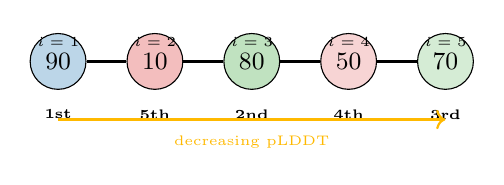
\begin{tikzpicture}[scale=0.82, every node/.style={font=\small}]
        % 5-node path graph
        \def\step{1.5}
        % Step 0: show all nodes labelled by pLDDT
        \node[draw, circle, fill=highhp!30, minimum size=0.7cm] (v1) at (0,0)     {90};
        \node[draw, circle, fill=lowhp!30,  minimum size=0.7cm] (v2) at (\step,0) {10};
        \node[draw, circle, fill=mixhp!30,  minimum size=0.7cm] (v3) at (2*\step,0){80};
        \node[draw, circle, fill=lowhp!20,  minimum size=0.7cm] (v4) at (3*\step,0){50};
        \node[draw, circle, fill=mixhp!20,  minimum size=0.7cm] (v5) at (4*\step,0){70};
        \draw[thick] (v1)--(v2)--(v3)--(v4)--(v5);
        \node[font=\tiny, above=2pt] at (v1) {$i=1$};
        \node[font=\tiny, above=2pt] at (v2) {$i=2$};
        \node[font=\tiny, above=2pt] at (v3) {$i=3$};
        \node[font=\tiny, above=2pt] at (v4) {$i=4$};
        \node[font=\tiny, above=2pt] at (v5) {$i=5$};
        % Insertion order arrow
        \node[font=\tiny, below=14pt] at (v1) {\textbf{1st}};
        \node[font=\tiny, below=14pt] at (v3) {\textbf{2nd}};
        \node[font=\tiny, below=14pt] at (v5) {\textbf{3rd}};
        \node[font=\tiny, below=14pt] at (v4) {\textbf{4th}};
        \node[font=\tiny, below=14pt] at (v2) {\textbf{5th}};
        \draw[->, thick, accentgold] (0,-0.9) -- (4*\step,-0.9)
          node[midway, below=2pt, font=\tiny] {decreasing pLDDT};
      \end{tikzpicture}
      \vspace{6pt}

      \footnotesize Numbers = pLDDT. Insertion order = by decreasing pLDDT.
    \end{column}
  \end{columns}
\end{frame}

\begin{frame}{Connected components, Elder Rule, and Persistence Diagram}
  \begin{columns}[T]
    \begin{column}{0.50\textwidth}
      \textbf{$N_{cc}(u)$}: number of connected components at level $u$
      \begin{itemize}
        \item New vertex inserted $\Rightarrow$ $N_{cc} +1$
        \item Edge joins two components $\Rightarrow$ $N_{cc} -1$
      \end{itemize}
      \vspace{4pt}
      \textbf{Elder Rule}: when two components merge,\\
      the one born at \emph{higher} pLDDT (older) survives.\\
      The younger one \textbf{dies}, producing a pair:
      \[
        (b_i,\, d_i) \quad b_i \geq d_i \geq 0
      \]
      \textbf{Persistence}: $p_i = b_i - d_i$\\
      \textbf{Accretion}: $p_i = 0$ (same-level merge)
      \vspace{4pt}

      \begin{block}{Persistence Diagram (PD)}
        Collection of all $m = n-1$ pairs
        $\mathcal{P} = \{(b_i, d_i)\}_{i=1}^{n-1}$
      \end{block}
    \end{column}
    \begin{column}{0.47\textwidth}
      \footnotesize
      \textbf{Toy example}: pLDDT $= [90, 10, 80, 50, 70]$\\[4pt]
      \begin{tabular}{@{}lll@{}}
        \toprule
        Event & $N_{cc}$ & PD pair \\
        \midrule
        Insert $i=1$ (90) & 1 & — \\
        Insert $i=3$ (80) & 2 & — \\
        Insert $i=5$ (70) & 3 & — \\
        Insert $i=4$ (50), edge $(4,5)$ & 3 & $(70, 50)$ \\
        edge $(3,4)$      & 2 & $(80, 50)$ \\
        Insert $i=2$ (10), edge $(1,2)$ & 2 & $(10,10)^\dagger$ \\
        edge $(2,3)$      & 1 & $(10,10)^\dagger$ \\
        \bottomrule
      \end{tabular}\\[4pt]
      $^\dagger$Accretions — zero persistence\\[6pt]
      Positive persistence pairs: $(70,50)$ and $(80,50)$
    \end{column}
  \end{columns}
\end{frame}

\begin{frame}{Five topological statistics}
  \begin{columns}[T]
    \begin{column}{0.48\textwidth}
      Let $m=n{-}1$, $m'=$ positive-persistence pairs,\\
      $\mathcal{P}_D=$ set of distinct persistence values.
      \vspace{2pt}

      \begin{enumerate}\setlength{\itemsep}{0pt}\setlength{\parsep}{0pt}
        \item $\displaystyle f^+_{cp} = \frac{m'}{n-1}$\\
              \emph{Fraction of heterogeneous transitions}
        \vspace{2pt}
        \item $\displaystyle \bar{p} = \frac{1}{m}\sum_i (b_i - d_i)$\\
              \emph{Mean persistence lifetime}
        \vspace{2pt}
        \item $\displaystyle H_p = \frac{-\sum_{v} \mathbb{P}[v]\ln\mathbb{P}[v]}{\ln|\mathcal{P}_D|}$\\
              \emph{Normalised Shannon entropy of persistence}\\
              $H_p \in [0,1]$; high $=$ diverse pLDDT profile
        \vspace{2pt}
        \item $N_{cc}^{max} = \max_u N_{cc}(u)$\\
              \emph{Peak simultaneous fragmentation}
        \vspace{2pt}
        \item $\mathrm{PLM}(t_p)$: persistent local maxima of $N_{cc}$\\
              \emph{Number of significant domain peaks}
      \end{enumerate}
    \end{column}
    \begin{column}{0.48\textwidth}
      % Ncc curve — pure TikZ, x-axis: 0=pLDDT100, 100=pLDDT0; y:0-5.5
      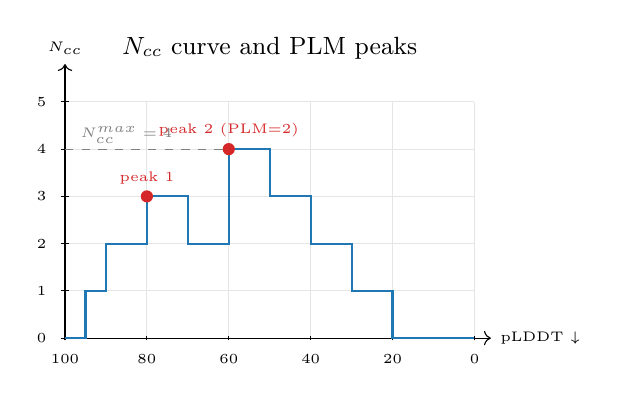
\begin{tikzpicture}[x=0.052cm, y=0.60cm]
        % Light grid
        \foreach \x in {20,40,60,80,100}
          \draw[gray!20,thin] (\x,0) -- (\x,5);
        \foreach \y in {1,2,3,4,5}
          \draw[gray!20,thin] (0,\y) -- (100,\y);
        % Axes
        \draw[->] (-0.5,0) -- (104,0) node[right,font=\tiny] {pLDDT $\downarrow$};
        \draw[->] (0,-0.05) -- (0,5.8) node[above,font=\tiny] {$N_{cc}$};
        % X ticks (labels reversed: axis 0 = pLDDT 100)
        \foreach \x/\l in {0/100,20/80,40/60,60/40,80/20,100/0} {
          \draw (\x,-0.05) -- (\x,0.05);
          \node[font=\tiny,below=1pt] at (\x,-0.08) {\l};
        }
        % Y ticks
        \foreach \y in {0,1,2,3,4,5} {
          \draw (-1,\y) -- (1,\y);
          \node[font=\tiny,left=1pt] at (-1.5,\y) {\y};
        }
        % Step-function curve (const plot equivalent)
        \draw[thick,highhp]
          (0,0)--(5,0)--(5,1)--(10,1)--(10,2)--(20,2)--(20,3)--(30,3)--(30,2)
          --(40,2)--(40,4)--(50,4)--(50,3)--(60,3)--(60,2)--(70,2)--(70,1)
          --(80,1)--(80,0)--(100,0);
        % Peak marks
        \fill[lowhp] (20,3) circle (2.2pt);
        \fill[lowhp] (40,4) circle (2.2pt);
        % Annotations
        \node[font=\tiny,lowhp,right=1pt,above=1pt] at (20,3) {peak 1};
        \node[font=\tiny,lowhp,right=1pt,above=1pt] at (40,4) {peak 2 (PLM=2)};
        % Ncc_max line
        \draw[dashed,gray,thin] (0,4) -- (40,4);
        \node[font=\tiny,gray] at (15,4.3) {$N_{cc}^{max}=4$};
        % Title
        \node[font=\small,anchor=south] at (50,5.7) {$N_{cc}$ curve and PLM peaks};
      \end{tikzpicture}
      \vspace{-6pt}

      \footnotesize PLM$\,\geq 3$ at $t_p = 0.025$ flags a protein as a
      \textbf{multi-domain fragmentation candidate}.
    \end{column}
  \end{columns}
\end{frame}

% =============================================================================
\section{Pipeline and Algorithm}
% =============================================================================

\begin{frame}{End-to-end pipeline overview}
  \begin{center}
  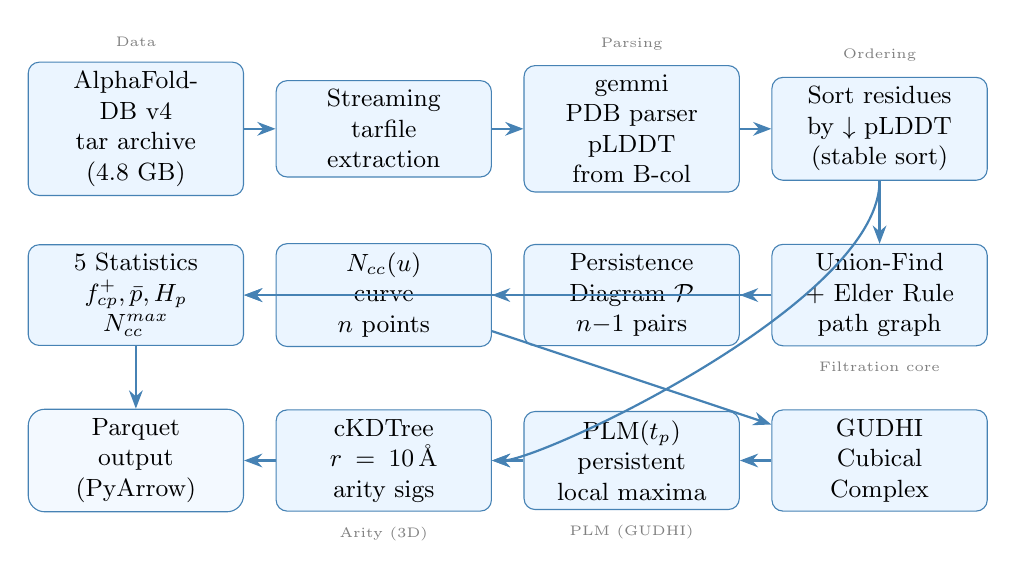
\begin{tikzpicture}[
    node distance = 0.55cm and 0.4cm,
    box/.style = {
      draw=pipeboxborder, fill=pipeboxbg, rounded corners=4pt,
      minimum width=2.6cm, minimum height=0.85cm,
      align=center, font=\small, text width=2.5cm
    },
    bigbox/.style = {
      draw=pipeboxborder, fill=pipeboxbg!60, rounded corners=6pt,
      minimum width=2.6cm, minimum height=0.85cm,
      align=center, font=\small, text width=2.5cm
    },
    arr/.style = {-Stealth, thick, pipeboxborder},
    label/.style = {font=\tiny, gray, align=center},
  ]
    % Row 1: data ingestion
    \node[box] (tar)  {AlphaFold-DB v4\\tar archive\\(4.8 GB)};
    \node[box, right=of tar]  (stream)  {Streaming\\tarfile\\extraction};
    \node[box, right=of stream] (gemmi)   {gemmi\\PDB parser\\pLDDT from B-col};
    \node[box, right=of gemmi]  (sort)    {Sort residues\\by $\downarrow$ pLDDT\\(stable sort)};

    % Row 2: filtration core
    \node[box, below=0.8cm of sort]  (uf)    {Union-Find\\+ Elder Rule\\path graph};
    \node[box, left=of uf]    (pd)    {Persistence\\Diagram $\mathcal{P}$\\$n{-}1$ pairs};
    \node[box, left=of pd]    (ncc)   {$N_{cc}(u)$\\curve\\$n$ points};
    \node[box, left=of ncc]   (stats) {5 Statistics\\$f^+_{cp}, \bar{p}, H_p$\\$N_{cc}^{max}$};

    % Row 3: PLM + arity + output
    \node[box, below=0.8cm of uf]    (gudhi)  {GUDHI\\Cubical\\Complex};
    \node[box, left=of gudhi]  (plm)   {PLM$(t_p)$\\persistent\\local maxima};
    \node[box, left=of plm]    (kd)    {cKDTree\\$r=10$\,\AA\\arity sigs};
    \node[bigbox, left=of kd]  (pq)    {Parquet\\output\\(PyArrow)};

    % Arrows row 1
    \draw[arr] (tar)    -- (stream);
    \draw[arr] (stream) -- (gemmi);
    \draw[arr] (gemmi)  -- (sort);
    \draw[arr] (sort)   -- (uf);

    % Arrows row 2
    \draw[arr] (uf)   -- (pd);
    \draw[arr] (uf)   -- (ncc);
    \draw[arr] (pd)   -- (stats);
    \draw[arr] (ncc)  -- (stats);

    % Arrows row 3
    \draw[arr] (ncc)   -- (gudhi);
    \draw[arr] (gudhi) -- (plm);
    \draw[arr] (sort) .. controls +(0,-2.2) and +(2,0) .. (kd);
    \draw[arr] (plm)  -- (kd);
    \draw[arr] (kd)   -- (pq);
    \draw[arr] (stats.south) -- ++(0,-0.35) -| (pq.north);

    % Labels
    \node[label, above=2pt of tar]    {Data};
    \node[label, above=2pt of gemmi]  {Parsing};
    \node[label, above=2pt of sort]   {Ordering};
    \node[label, below=2pt of uf]     {Filtration core};
    \node[label, below=2pt of plm]    {PLM (GUDHI)};
    \node[label, below=2pt of kd]     {Arity (3D)};
  \end{tikzpicture}
  \end{center}
  \vspace{2pt}
  {\footnotesize 6 parallel workers via \texttt{multiprocessing.Pool} — processes 23\,391 proteins in $\approx$30 seconds.}
\end{frame}

\begin{frame}{Algorithm: standard sublevel-set filtration}
  \begin{block}{\footnotesize\bfseries Path-graph pLDDT filtration (paper-faithful)}
  \footnotesize
  \textbf{Input:} $(s_1,\ldots,s_n)$, threshold $t_p$\quad
  \textbf{Output:} $\mathcal{P}$, $N_{cc}$-curve, PLM$(t_p)$
  \begin{enumerate}\setlength{\itemsep}{1pt}\setlength{\parskip}{0pt}
    \item $\pi \gets \textsc{StableArgsort}(-s)$ \hfill\textit{decreasing pLDDT; ties by index}
    \item Init UF: $\mathrm{parent}[i]\!\gets\!i$, $\mathrm{birth}[i]\!\gets\!-\infty$, $\mathrm{inserted}[i]\!\gets\!\bot$;\quad $N_{cc}\!\gets\!0$
    \item \textbf{for each} $i$ in $\pi$:\;
          $\mathrm{birth}[i]\!\gets\!s_i$;\; $\mathrm{inserted}[i]\!\gets\!\top$;\; $N_{cc}\!\gets\!N_{cc}+1$
          \begin{itemize}\setlength{\itemsep}{0pt}
            \item \textbf{for} $j\in\{i{-}1,i{+}1\}$ with $\mathrm{inserted}[j]$; let $r_i,r_j=\textsc{Find}(i,j)$:
            \begin{itemize}\setlength{\itemsep}{0pt}
              \item $r_i=r_j$: append $(s_i,s_i)$ \hfill(accretion)
              \item else (\textbf{Elder Rule}): survivor $=\arg\max\mathrm{birth}$;\;
                    merge loser$\to$survivor;\; $N_{cc}\!-\!=\!1$;\;
                    append $(\mathrm{birth}[\text{loser}],\,s_i)$
            \end{itemize}
            \item append $(s_i,\,N_{cc})$ to Curve
          \end{itemize}
    \item $\mathrm{PLM}(t_p)\gets\textsc{GUDHIPersistentMaxima}(\text{Curve},\;t_\nu\!=\!n\cdot t_p)$
    \item \textbf{return} $\mathcal{P}$, Curve, PLM$(t_p)$
  \end{enumerate}
  \end{block}
  \vspace{2pt}
  {\footnotesize \textsc{Find} uses path-halving ($O(\alpha(n))\approx O(1)$).
  GUDHI step: negate $N_{cc}$, 1D cubical complex, count 0-dim pairs with persistence $\geq t_\nu$.}
\end{frame}

\begin{frame}{PLM via GUDHI — second-layer persistence}
  \begin{columns}[T]
    \begin{column}{0.52\textwidth}
      The $N_{cc}$ curve is itself a 1D scalar function.\\
      Its local maxima correspond to \textbf{pLDDT domain peaks}.
      \vspace{6pt}

      \textbf{How we count significant peaks:}
      \begin{enumerate}
        \item Negate $N_{cc}$: local maxima become local \emph{minima}
        \item Feed $-N_{cc}$ to GUDHI's \texttt{CubicalComplex}
        \item Each 0-dim pair $(b_j, d_j)$ in the resulting PD has
              persistence $= N_{cc}[\text{peak}] - N_{cc}[\text{valley}]$
        \item Count pairs with persistence $\geq t_\nu = n \cdot t_p$
      \end{enumerate}
      \vspace{6pt}

      \textbf{Why two layers of persistence?}\\
      First layer: filtration of the \emph{protein graph}.\\
      Second layer: Morse-Smale simplification of the
      \emph{$N_{cc}$ function} — filters out noise peaks from
      float-precision pLDDT.
    \end{column}
    \begin{column}{0.44\textwidth}
      % Ncc multi-domain curve — pure TikZ, x:0-56 y:0-6
      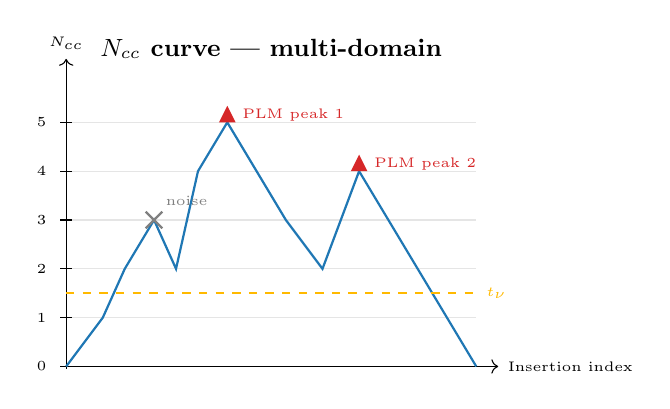
\begin{tikzpicture}[x=0.093cm, y=0.62cm]
        % Light grid
        \foreach \y in {1,2,3,4,5}
          \draw[gray!20,thin] (0,\y) -- (56,\y);
        % Axes
        \draw[->] (-0.5,0) -- (59,0) node[right,font=\tiny] {Insertion index};
        \draw[->] (0,-0.05) -- (0,6.3) node[above,font=\tiny] {$N_{cc}$};
        % Y ticks
        \foreach \y in {0,1,2,3,4,5} {
          \draw (-0.8,\y) -- (0.8,\y);
          \node[font=\tiny,left=1pt] at (-1,\y) {\y};
        }
        % Curve
        \draw[thick,highhp] plot coordinates
          {(0,0)(5,1)(8,2)(12,3)(15,2)(18,4)(22,5)(26,4)
           (30,3)(35,2)(40,4)(44,3)(48,2)(52,1)(56,0)};
        % Persistent peaks (filled triangles via polygon)
        \fill[lowhp] (22,5) +(-3pt,0) -- +(3pt,0) -- +(0,6pt) -- cycle;
        \fill[lowhp] (40,4) +(-3pt,0) -- +(3pt,0) -- +(0,6pt) -- cycle;
        % Noise (cross mark)
        \draw[gray,thick] (12,3) +(-3pt,-3pt) -- +(3pt,3pt);
        \draw[gray,thick] (12,3) +(-3pt,3pt) -- +(3pt,-3pt);
        % Labels
        \node[font=\tiny,lowhp,right=2pt] at (22,5.15) {PLM peak 1};
        \node[font=\tiny,lowhp,right=2pt] at (40,4.15) {PLM peak 2};
        \node[font=\tiny,gray,above right=1pt] at (12,3.05) {noise};
        % t_nu threshold
        \draw[dashed,accentgold,thick] (0,1.5) -- (56,1.5)
          node[right,font=\tiny,accentgold] {$t_\nu$};
        % Title
        \node[font=\small\bfseries,anchor=south] at (28,6.1)
          {$N_{cc}$ curve --- multi-domain};
      \end{tikzpicture}
    \end{column}
  \end{columns}
\end{frame}

% =============================================================================
\section{Arity Extension (Q1 × Q4)}
% =============================================================================

\begin{frame}{Arity: a 3D packing descriptor}
  \begin{columns}[T]
    \begin{column}{0.52\textwidth}
      \textbf{Arity of residue $k$}:\\
      \# of $\mathrm{C}_\alpha$ atoms within 10\,\AA\ of $\mathrm{C}_\alpha(k)$
      (excluding self)
      \vspace{6pt}

      \textbf{Arity signature} $(a_{25}, a_{75})$:\\
      25th and 75th percentiles of per-residue arity
      \begin{itemize}
        \item $a_{25}$ low $\Rightarrow$ flexible/disordered regions dominate
        \item $a_{75}$ high $\Rightarrow$ well-packed globular regions present
        \item Multi-domain proteins: \emph{both} — compact domains
              + disordered linkers
      \end{itemize}
      \vspace{6pt}

      \textbf{Implementation:}
      \begin{itemize}
        \item Extract $\mathrm{C}_\alpha$ coordinates (gemmi)
        \item Build \texttt{scipy.cKDTree}
        \item \texttt{query\_ball\_point(r=10)} — $O(n\log n)$
        \item Subtract 1 for self-count
      \end{itemize}
    \end{column}
    \begin{column}{0.45\textwidth}
      % Arity map schematic — pure TikZ, x:0-18 y:0-22
      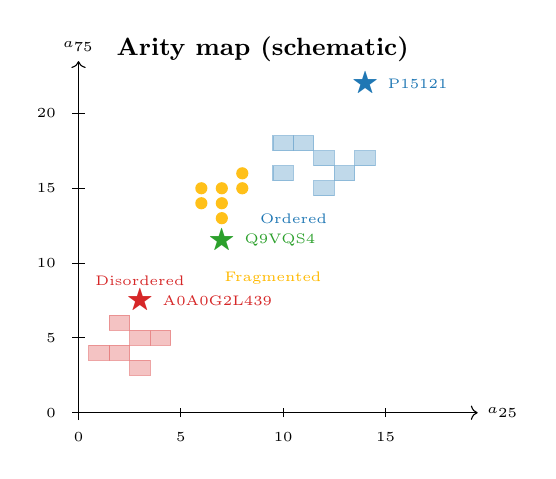
\begin{tikzpicture}[x=0.26cm, y=0.19cm]
        % Axes
        \draw[->] (-0.3,0) -- (19.5,0) node[right,font=\tiny] {$a_{25}$};
        \draw[->] (0,-0.5) -- (0,23.5) node[above,font=\tiny] {$a_{75}$};
        % X ticks
        \foreach \x in {0,5,10,15} {
          \draw (\x,-0.3) -- (\x,0.3);
          \node[font=\tiny,below=1pt] at (\x,-0.5) {\x};
        }
        % Y ticks
        \foreach \y in {0,5,10,15,20} {
          \draw (-0.3,\y) -- (0.3,\y);
          \node[font=\tiny,left=1pt] at (-0.5,\y) {\y};
        }
        % Ordered blob (high arity — blue squares)
        \foreach \xx/\yy in {10/16,12/17,11/18,13/16,10/18,12/15,14/17}
          \fill[highhp!40,draw=highhp!60,opacity=0.7]
            (\xx-0.5,\yy-0.5) rectangle (\xx+0.5,\yy+0.5);
        % Disordered blob (low arity — red squares)
        \foreach \xx/\yy in {2/4,3/5,1/4,2/6,3/3,4/5}
          \fill[lowhp!40,draw=lowhp!60,opacity=0.7]
            (\xx-0.5,\yy-0.5) rectangle (\xx+0.5,\yy+0.5);
        % Fragmented candidates (gold dots)
        \foreach \xx/\yy in {7/15,6/14,8/16,7/14,6/15,8/15,7/13}
          \fill[accentgold,opacity=0.9] (\xx,\yy) circle (2.2pt);
        % Prototype stars
        \node[highhp,font=\normalsize] at (14,22) {$\bigstar$};
        \node[font=\tiny,highhp,right=1pt] at (14.5,22) {P15121};
        \node[lowhp,font=\normalsize] at (3,7.5) {$\bigstar$};
        \node[font=\tiny,lowhp,right=1pt] at (3.5,7.5) {A0A0G2L439};
        \node[mixhp,font=\normalsize] at (7,11.5) {$\bigstar$};
        \node[font=\tiny,mixhp,right=1pt] at (7.5,11.5) {Q9VQS4};
        % Legend labels
        \node[font=\tiny,highhp] at (10.5,13) {Ordered};
        \node[font=\tiny,lowhp]  at (3,8.8)   {Disordered};
        \node[font=\tiny,accentgold] at (9.5,9) {Fragmented};
        % Title
        \node[font=\small\bfseries,anchor=south] at (9,22.8) {Arity map (schematic)};
      \end{tikzpicture}
    \end{column}
  \end{columns}
\end{frame}

% =============================================================================
\section{Validation}
% =============================================================================

\begin{frame}{Validation: toy example and null model}
  \begin{columns}[T]
    \begin{column}{0.48\textwidth}
      \textbf{Toy protein} ($n=5$, pLDDT $= [10, 90, 80, 90, 10]$)
      \vspace{4pt}

      \begin{tabular}{@{}lll@{}}
        \toprule
        Pair & $(b_i, d_i)$ & Type \\
        \midrule
        $(80, 80)$ & accretion & \\
        $(90, 80)$ & $p=10$ & positive \\
        $(10, 10)$ & accretion & \\
        $(10, 10)$ & accretion & \\
        \bottomrule
      \end{tabular}
      \vspace{6pt}

      Hand-computed:
      \[
        H_p = 0.8112, \quad f^+_{cp} = 0.25
      \]
      Code output (4 d.p.):
      \[
        H_p = 0.8113, \quad f^+_{cp} = 0.25 \;\checkmark
      \]
    \end{column}
    \begin{column}{0.48\textwidth}
      \textbf{Null random model} ($n=1{,}000$,
      pLDDT $\sim \mathcal{U}[0,100]$)\\[4pt]

      Cazals \& Sarti (2025) Example~1:
      \begin{itemize}
        \item $f^+_{cp} \approx 1/3 = 0.333$
        \item $H_p \approx 0.45$
        \item $N_{cc}^{max} \approx n/4 = 250$
      \end{itemize}
      \vspace{6pt}

      Our result (raw float pLDDT):
      \begin{itemize}
        \item $f^+_{cp} = 0.329$ \;\checkmark
        \item $H_p = 0.438$ \;\checkmark
        \item $N_{cc}^{max} = 252$ \;\checkmark
      \end{itemize}
      \vspace{4pt}
      \footnotesize Note: despite continuous float inputs, only 330 distinct
      persistence values arise, keeping $H_p \ll 1$.
    \end{column}
  \end{columns}
\end{frame}

\begin{frame}{Validation: three prototype proteins}
  \begin{columns}[T]
    \begin{column}{0.50\textwidth}
      \begin{tabular}{@{}llrrrr@{}}
        \toprule
        UniProt & Type & $n$ & $H_p$ & $f^+_{cp}$ & PLM \\
        \midrule
        \multicolumn{6}{l}{\textit{Paper targets (Fig.~3)}} \\
        P15121 & Ordered & 316 & $\approx$0.04 & — & — \\
        A0A0G2L439 & Disord. & 449 & $\approx$0.27 & — & — \\
        Q9VQS4 & Mixed & 781 & $\approx$0.28 & — & — \\
        \midrule
        \multicolumn{6}{l}{\textit{Our results (raw float pLDDT)}} \\
        P15121 & Ordered & 316 & 0.371 & 0.241 & 1 \\
        A0A0G2L439 & Disord. & 449 & 0.466 & 0.339 & 1 \\
        Q9VQS4 & Mixed & 781 & 0.424 & 0.312 & 2 \\
        \bottomrule
      \end{tabular}
      \vspace{6pt}

      \textbf{Key:} relative ordering preserved\\
      Ordered $<$ Mixed $<$ Disordered \;\checkmark
    \end{column}
    \begin{column}{0.47\textwidth}
      \hspace{0.9cm}\textbf{Why are our $H_p$ values higher?}
      \vspace{4pt}

      \hspace{0.9cm}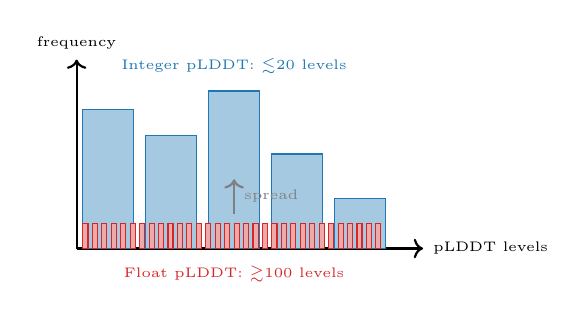
\begin{tikzpicture}[scale=0.8]
        \draw[thick, ->] (0,0) -- (5.5,0) node[right, font=\tiny] {pLDDT levels};
        \draw[thick, ->] (0,0) -- (0,3) node[above, font=\tiny] {frequency};
        % Integer pLDDT (few broad bars)
        \foreach \x/\h in {0.5/2.2, 1.5/1.8, 2.5/2.5, 3.5/1.5, 4.5/0.8} {
          \fill[highhp!40, draw=highhp] (\x-0.4,0) rectangle (\x+0.4,\h);
        }
        \node[font=\tiny, highhp] at (2.5,2.9) {Integer pLDDT: $\lesssim$20 levels};
        % Float pLDDT (many thin bars)
        \foreach \x in {0.1,0.25,0.4,0.55,0.7,0.85,1.0,1.15,1.3,...,4.9} {
          \fill[lowhp!40, draw=lowhp] (\x,0) rectangle (\x+0.08, 0.4);
        }
        \node[font=\tiny, lowhp] at (2.5,-0.4) {Float pLDDT: $\gtrsim$100 levels};
        % Arrow
        \draw[->, thick, gray] (2.5, 0.55) -- (2.5, 1.1)
          node[midway, right, font=\tiny, gray] {spread};
      \end{tikzpicture}

      \vspace{4pt}
      \hspace{0.9cm}\begin{minipage}{0.85\linewidth}
      \footnotesize More distinct pLDDT levels $\to$ more distinct persistence
      values $\to$ broader $\mathbb{P}[v]$ $\to$ higher $H_p$.
      \end{minipage}
    \end{column}
  \end{columns}
\end{frame}

% =============================================================================
\section{Proteome-Scale Results}
% =============================================================================

\begin{frame}{Proteome-scale Pearson correlation (Figure 7)}
  \begin{columns}[T]
    \begin{column}{0.55\textwidth}
      \includegraphics[width=\textwidth, height=6.6cm, keepaspectratio]{../data/results/figure7_full.png}
    \end{column}
    \begin{column}{0.42\textwidth}
      \vspace{2pt}
      \textbf{Setup}: all 23\,391 AlphaFold-DB v4 fragments\\
      No length pre-filter (paper-faithful)
      \vspace{4pt}

      \begin{tabular}{@{}lr@{}}
        \toprule
        Metric & Value \\
        \midrule
        $N$ & 23\,391 \\
        Pearson $r$ & \textbf{0.864} \\
        Paper target & $\approx 0.97$ \\
        Gap & $-0.106$ \\
        \bottomrule
      \end{tabular}
      \vspace{4pt}

      \textbf{Both statistics elevated} (diagonal shift)\\
      $\to$ slope preserved, variance increased\\
      $\to$ $r$ reduced by float-precision effect
      \vspace{4pt}

      \footnotesize Median $f^+_{cp} = 0.242$,
      Median $H_p = 0.362$
    \end{column}
  \end{columns}
\end{frame}

\begin{frame}{Fragmentation candidates and $t_p$ sensitivity}
  \begin{columns}[T]
    \begin{column}{0.50\textwidth}
      \textbf{Three-way filter} (paper's Fig.~8):
      \[
        n \geq 200,\quad H_p \geq 0.25,\quad \mathrm{PLM}(t_p) \geq 3
      \]
      \vspace{4pt}

      \begin{tabular}{@{}rrr@{}}
        \toprule
        $t_p$ & Candidates & Paper \\
        \midrule
        0.020 & 822 & — \\
        \textbf{0.025} & \textbf{183} & $\approx$\textbf{86} \\
        0.030 &  34 & — \\
        \bottomrule
      \end{tabular}
      \vspace{10pt}

      \textbf{Why 183 instead of 86?}\\
      Float pLDDT creates many fine-grained\\
      $N_{cc}$ oscillations $\to$ more peaks\\
      clear the threshold $t_\nu = 0.025 \cdot n$

      \vspace{6pt}
      34 proteins survive all thresholds\\
      = \textbf{robust, threshold-independent core}
    \end{column}
    \begin{column}{0.47\textwidth}
      \includegraphics[width=\textwidth]{../data/results/figure8a_scatter.png}
      \vspace{-4pt}

      \footnotesize\centering 3D scatter: length $\times$ $H_p$ $\times$ $f^+_{cp}$.
      Orange = fragmentation candidates.
    \end{column}
  \end{columns}
\end{frame}

\begin{frame}{Q1 × Q4 cross-correlation}
  \begin{columns}[T]
    \begin{column}{0.52\textwidth}
      \includegraphics[width=\textwidth]{../data/results/figure_q1q4_overlay.png}
    \end{column}
    \begin{column}{0.45\textwidth}
      \vspace{2pt}
      \textbf{Finding}: fragmented proteins (PLM$\,\geq 3$) cluster in a
      specific arity bin

      \vspace{2pt}
      \begin{tabular}{@{}ll@{}}
        \toprule
        Property & Value \\
        \midrule
        Centroid & $(a_{25}=7,\; a_{75}=15)$ \\
        Enrichment & \textbf{5.92×} \\
        $p$-value & $1.61\times10^{-3}$ \\
        Test & Fisher exact \\
        \bottomrule
      \end{tabular}
      \vspace{3pt}

      \textbf{Biological interpretation}
      \begin{itemize}\setlength{\itemsep}{0pt}\setlength{\parsep}{0pt}
        \item $a_{25}\approx7$: disordered linkers with few contacts
        \item $a_{75}\approx15$: well-packed domain cores
        \item Intermediate arity = mix of compact domains + disordered linkers
              = \textbf{multi-domain hallmark}
      \end{itemize}

      \vspace{0pt}
      \footnotesize This finding is \emph{orthogonal} to pLDDT — derived
      purely from 3D $\mathrm{C}_\alpha$ coordinates.
    \end{column}
  \end{columns}
\end{frame}

% =============================================================================
\section{Discussion}
% =============================================================================

\begin{frame}{The float-precision gap — unified explanation}
  \begin{center}
  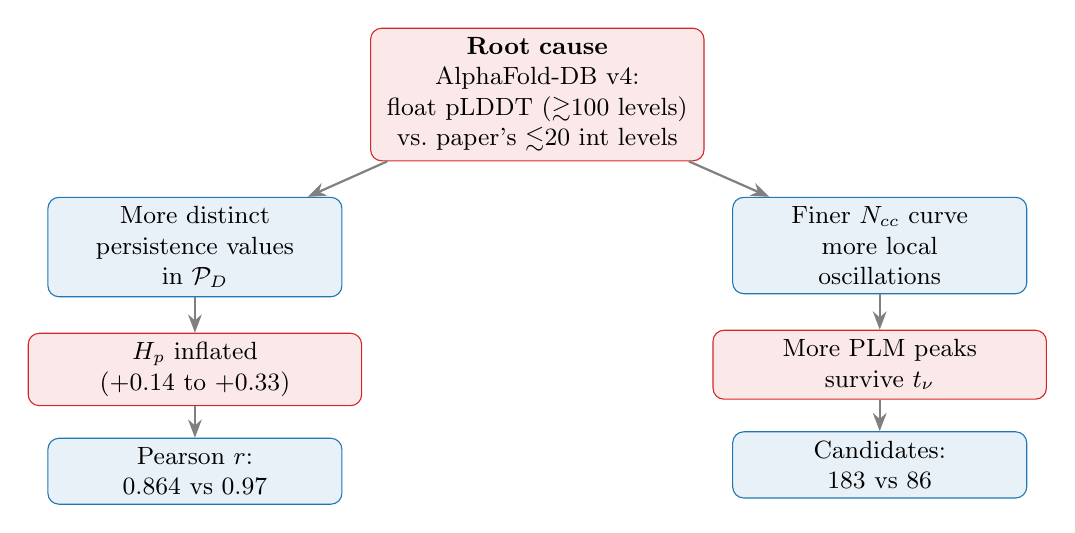
\begin{tikzpicture}[
    node distance=0.45cm and 0.4cm,
    cause/.style={draw=lowhp, fill=lowhp!10, rounded corners=4pt,
                  minimum width=4cm, minimum height=0.65cm,
                  align=center, font=\small, text width=4cm},
    effect/.style={draw=highhp, fill=highhp!10, rounded corners=4pt,
                   minimum width=3.6cm, minimum height=0.65cm,
                   align=center, font=\small, text width=3.5cm},
    arr/.style={-Stealth, thick, gray},
  ]
    \node[cause] (root) {\textbf{Root cause}\\AlphaFold-DB v4:\\float pLDDT ($\gtrsim$100 levels)\\vs.\ paper's $\lesssim$20 int levels};
    \node[effect, below left=0.45cm and 0.35cm of root]  (e1) {More distinct\\persistence values\\in $\mathcal{P}_D$};
    \node[effect, below right=0.45cm and 0.35cm of root] (e2) {Finer $N_{cc}$ curve\\more local\\oscillations};
    \node[cause, below=0.45cm of e1]  (c1) {$H_p$ inflated\\(+0.14 to +0.33)};
    \node[cause, below=0.45cm of e2]  (c2) {More PLM peaks\\survive $t_\nu$};
    \node[effect, below=0.40cm of c1] (r1) {Pearson $r$:\\0.864 vs 0.97};
    \node[effect, below=0.40cm of c2] (r2) {Candidates:\\183 vs 86};

    \draw[arr] (root) -- (e1);
    \draw[arr] (root) -- (e2);
    \draw[arr] (e1) -- (c1);
    \draw[arr] (e2) -- (c2);
    \draw[arr] (c1) -- (r1);
    \draw[arr] (c2) -- (r2);
  \end{tikzpicture}
  \end{center}
  \vspace{1pt}
  {\small Both gaps share a single falsifiable hypothesis: reproducing the analysis
  on integer-rounded pLDDT would close them — at the cost of departing from
  the paper's stated methodology.}
\end{frame}

\begin{frame}{AlphaFold-DB v6 replication: gap persists}
  \begin{columns}[T]
    \begin{column}{0.52\textwidth}
      \textbf{Question}: does v6 close the gap with the paper?\\[5pt]
      Full pipeline re-run on v6 tarball (5.1\,GB, May~2026)\\
      23{,}586 proteins processed, 0 failures\\[6pt]

      \begin{tabular}{@{}lrrr@{}}
        \toprule
        Metric & v4 & v6 & $\Delta$ \\
        \midrule
        $N$ proteins           & 23{,}391 & 23{,}586 & $+195$   \\
        Pearson $r$            & 0.864    & 0.862    & $-0.002$ \\
        Median $f^+_{cp}$      & 0.242    & 0.239    & $-0.003$ \\
        Median $H_p$           & 0.362    & 0.359    & $-0.003$ \\
        Candidates$^\dagger$   & 183      & 185      & $+2$     \\
        \bottomrule
      \end{tabular}\\[3pt]
      \footnotesize $^\dagger$ $n\!\geq\!200$,
      $H_p\!\geq\!0.25$, PLM$(0.025)\!\geq\!3$
    \end{column}
    \begin{column}{0.45\textwidth}
      \vspace{4pt}
      \textbf{Answer: no.}\\[6pt]

      Both v4 and v6 store pLDDT as \textbf{float}\\
      $\to$ neither matches the paper's\\
      \hspace{1em}integer-quantised data\\[8pt]

      All statistics change by $<0.5\%$:
      \begin{itemize}\setlength{\itemsep}{2pt}
        \item $\Delta r = -0.002$
        \item $\Delta\,\text{candidates} = +2$
        \item $+195$ new UniProt entries\\
              (curation updates, not\\
              structural changes)
      \end{itemize}
      \vspace{6pt}

      \begin{block}{}
        The float-precision gap is an\\
        \textbf{AlphaFold-DB property},\\
        not a v4 artifact.
      \end{block}
    \end{column}
  \end{columns}
\end{frame}

\begin{frame}{Arity enrichment: biological significance}
  \begin{columns}[T]
    \begin{column}{0.48\textwidth}
      \textbf{What the enrichment tells us}
      \vspace{6pt}

      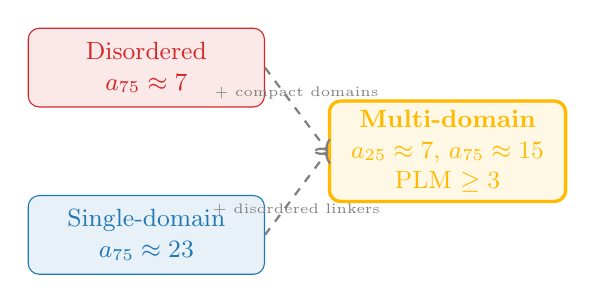
\begin{tikzpicture}[scale=0.85, every node/.style={font=\small}]
        % Three protein archetypes
        % Disordered
        \node[draw, lowhp, fill=lowhp!10, rounded corners=4pt,
              minimum width=3cm, minimum height=1cm, align=center]
          (dis) at (0, 2.5) {Disordered\\$a_{75}\approx7$};
        % Ordered
        \node[draw, highhp, fill=highhp!10, rounded corners=4pt,
              minimum width=3cm, minimum height=1cm, align=center]
          (ord) at (0, 0) {Single-domain\\$a_{75}\approx23$};
        % Multi-domain (fragmented)
        \node[draw, accentgold, fill=accentgold!10, rounded corners=4pt,
              minimum width=3cm, minimum height=1.1cm, align=center, very thick]
          (frag) at (4.5, 1.25) {\textbf{Multi-domain}\\$a_{25}\approx7$, $a_{75}\approx15$\\PLM $\geq 3$};
        % Arrows
        \draw[->, thick, gray, dashed] (dis.east) -- (frag.west)
          node[midway, above, font=\tiny, gray] {+ compact domains};
        \draw[->, thick, gray, dashed] (ord.east) -- (frag.west)
          node[midway, below, font=\tiny, gray] {+ disordered linkers};
      \end{tikzpicture}
    \end{column}
    \begin{column}{0.48\textwidth}
      \textbf{Two orthogonal signals agree:}
      \vspace{4pt}

      \begin{enumerate}
        \item \textbf{pLDDT fragmentation} (Q4):\\
              PLM$\,\geq 3$ identifies proteins with multiple
              confident domains separated by linkers
        \vspace{6pt}
        \item \textbf{$\mathrm{C}_\alpha$ arity} (Q1):\\
              Moderate $a_{25}$ (linkers) + moderate $a_{75}$ (domains)
              $\to$ same proteins
      \end{enumerate}
      \vspace{8pt}

      \textbf{Convergence of two independent structural descriptors}
      provides mutual validation and strengthens confidence in the
      topological fragmentation signal.
    \end{column}
  \end{columns}
\end{frame}

% =============================================================================
\section{Conclusions}
% =============================================================================

\begin{frame}{Summary}
  \begin{columns}[T]
    \begin{column}{0.50\textwidth}
      \textbf{What we reproduced}
      \begin{itemize}
        \item Full path-graph filtration from scratch\\
              (Union-Find + Elder Rule)
        \item All 5 statistics + PLM via GUDHI
        \item Applied to all 23\,391 H. sapiens\\
              AlphaFold-DB v4 fragments
        \item Pearson $r = 0.864$ vs target 0.97
        \item 183 fragmentation candidates vs target 86
        \item Relative ordering of prototypes preserved \checkmark
        \item Null model targets matched \checkmark
      \end{itemize}
    \end{column}
    \begin{column}{0.47\textwidth}
      \textbf{Novel extension (Q1 × Q4)}
      \begin{itemize}
        \item Proteome-wide arity signatures
        \item 5.92-fold enrichment of fragmented\\
              proteins at $(a_{25}=7, a_{75}=15)$
        \item $p = 1.61\times10^{-3}$ (Fisher exact)
        \item Orthogonal 3D validation of pLDDT\\
              fragmentation signal
      \end{itemize}
      \vspace{10pt}

      \textbf{Key insight}
      \begin{block}{}
        All discrepancies with the paper trace to
        a single cause: float vs.\ integer pLDDT
        in AlphaFold-DB v4 vs.\ the paper's data.
      \end{block}
    \end{column}
  \end{columns}
  \vspace{6pt}
  \begin{center}
    \footnotesize
    Code: Python 3.11 — NumPy · SciPy · gemmi · GUDHI · PyArrow
    · streaming tar pipeline (30 s for 23\,391 proteins)
  \end{center}
\end{frame}

\begin{frame}[plain]
  \begin{center}
    \vspace{0.3cm}
    {\Large\bfseries Thank you}\\[8pt]
    {\large Questions?}\\[10pt]
    \begin{tabular}{ll}
      Paper: & Cazals \& Sarti (2025), bioRxiv 2024.11.16.623929 \\
      Data:  & AlphaFold-DB v4 — \textit{H.~sapiens} proteome \\
    \end{tabular}
    \vspace{8pt}

    \includegraphics[width=0.38\textwidth]{../data/results/figure4_arity_map.png}
  \end{center}
\end{frame}

\end{document}
